\subsection{Signal Model}

\begin{frame}{Signal model}

    % Sound propagation process $\Leftrightarrow$ Source $\to$ Filter $\to$ Receiver model

    For one source and $I$ microphones:

    \begin{equation*}
        \tikzmarknode{x}{\contMic}_i(t)
                = (
                    \textcolor{orange}{\tikzmarknode{h}{\contRIR}_i}
                    \tikzmarknode{A}{\contConv}
                    \tikzmarknode{s}{\contSrc})(t)
                    + \tikzmarknode{n}{\contNse}_i(t)
                    \quad i \in I
    \end{equation*}

    \visible<2->{
    \vspace{10mm}
    \begin{mydefblock}{\tikzmarknode{RIR}{Room Impulse Response} (RIR)}
        \small
        \begin{itemize}
            \item linear filtering effect of the sound propagation (reverberation)
            \item acoustic response of a room to a (prefect) impulsive sound
            \item depends on spatial properties (room geometry, mic/src position)
            \\$\to$ one RIR for each microphone and source pair
        \end{itemize}
    \end{mydefblock}}

    \visible<3->{
    \begin{block}{}
        In the Short Time Fourier Transform (STFT) domain:
        \begin{equation*}
            X_i[f,t] = \tikzmarknode{H}{H}_i[f] S[f,t] + N_i[f,t]
        \end{equation*}
        where $X[f,t], H[f,t], S[f,t], N[f,t] \in \bbC$
    \end{block}}


    \begin{tikzpicture}[overlay,remember picture,
        nodes={inner sep=1pt, align=center, font=\footnotesize},
        gray!70,>=stealth] %
    \visible<1->{\draw[->] (x.north) to[out=90, in=0]   ++ (-8mm,+4mm) node[left] {{mic. signal}};}
    \visible<1->{\draw[->] (s.north) to[out=90, in=180] ++ (+8mm,+4mm) node[right] {{source signal}};}
    \visible<1->{\draw[->] (n.south) to[out=-90, in=180] ++ (+8mm,-4mm) node[right] {{noise term}};}
    \visible<1->{\draw[->] (A.south) to[out=-90, in=180] ++ (+8mm,-8mm) node[right] {{\faExclamationTriangle~continuous-time convolution}};}
    \visible<2->{\draw[->] (h.south) to[out=-90, in=90] (RIR.north);}
    \visible<3->{\draw[->] (H.south) to[out=-90, in=180] ++ (+8mm,-4mm) node[right] {{\alert{Room Transfer Function (RTF)}}};}
    \end{tikzpicture}

\end{frame}


\begin{frame}{Elements of RIR}
    \begin{columns}[T,onlytextwidth]
        \column{0.48\textwidth}
        \begin{equation*}
            \begin{aligned}
                \contMic_i(t) &= (\contRIR_i \contConv \contSrc)(t) + \contNse(t)\\
                \contRIR_i(t) &= \textcolor{myred}{\contRIRidirect}(t)
                              + \textcolor{myblue}{\contRIRiearly}(t)
                              + \textcolor{mygreen}{\contRIRilate}(t)

            \end{aligned}
        \end{equation*}
        \begin{itemize}\small
            \item<2-> $\textcolor{myred}{\contRIRidirect}(t)$ = direct path
            \item<3-> $\textcolor{myblue}{\contRIRiearly}(t)$ = early reflection
            \item<4-> $\textcolor{mygreen}{\contRIRilate}(t)$ = late reverberation
        \end{itemize}

        \column{0.48\textwidth}
        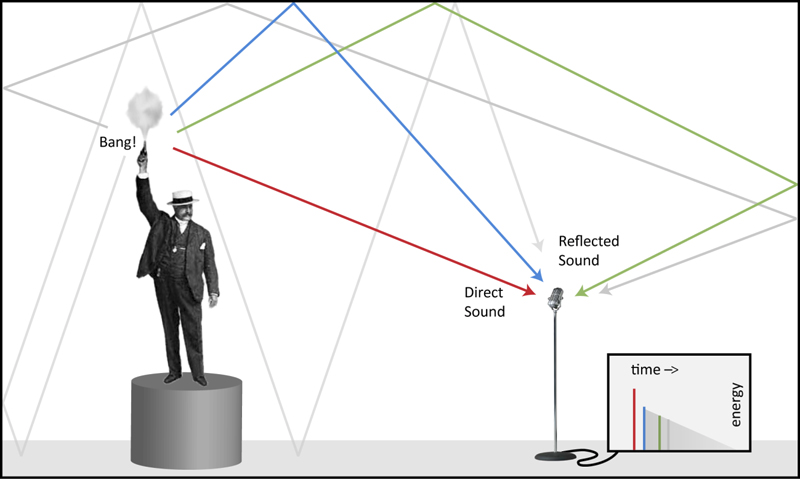
\includegraphics[width=.8\textwidth]{figures/rir_bang.png}
        \addendum{\footnoitesize \faCopyright[regular]~acousticshonoursproject}

    \end{columns}

    \begin{center}
        % real RIR with part
        \includegraphics<1>[width=0.8\textwidth]{figures/rir_elements0.pdf}%
        \includegraphics<2>[width=0.8\textwidth]{figures/rir_elements1.pdf}%
        \includegraphics<3>[width=0.8\textwidth]{figures/rir_elements2.pdf}%
        \includegraphics<4>[width=0.8\textwidth]{figures/rir_elements3.pdf}%
    \end{center}

\end{frame}

\subsection{Current Challenges}

\begin{frame}{Problem Statement}
    Echoes can be modeled as sum of Dirac's delta functions:

    \begin{equation*}
        \contRIR_i(t) =
            \textcolor{myred}{\contRIRidirect}(t) + \textcolor{myblue}{\contRIRiearly}(t) + \varepsilon_i(t)
            \approx \sum_{r=0}^{R} \ampir \delta\kparen{t - \textcolor{alert}{\tauir}} + \tikzmarknode{error}{\varepsilon}_i(t)
    \end{equation*}

    \begin{textblock*}{30mm}(100mm,35mm)
        \footnotesize
        \textcolor{gray}{\tikzmarknode{model}{models} later echoes, reverberation and other.}
    \end{textblock*}


    \begin{tikzpicture}[overlay,remember picture,
        nodes={inner sep=1pt, align=center, font=\footnotesize},
        gray!70,>=stealth] %
    \draw[->] (error.south) to[out=-90, in=180] (model.west);
    \end{tikzpicture}

    \pause

    \begin{mydefblock}{Goal: Acoustic Echo Retrieval (AER)}
        Estimate $\set{\tauir, \textcolor{gray}{\ampir_i}}_{i,r}$
        from the microphone signals $\set{x_i}_i$
    \end{mydefblock}
    % \addendum{\scriptsize {Estimation of only $\tauir$ is known as TOAs estimation}}

    \pause[3]
    \begin{block}{Challenges:}
        \begin{itemize}
            \item<4-> RIRs depend on the scene geometry (room, source and mic position)
            \item<5-> Big under-modelling error (late reverberation and external noise)
            \item<6-> In reality: $\ampir\delta(t) \to (\ampir\contConv\delta)(t)$ due to
            \begin{itemize}
                \item frequency-dependent air attenuation, wall absorption, ...
                \item sampling process
            \end{itemize}
        \end{itemize}
    \end{block}

    % \begin{center}
    %     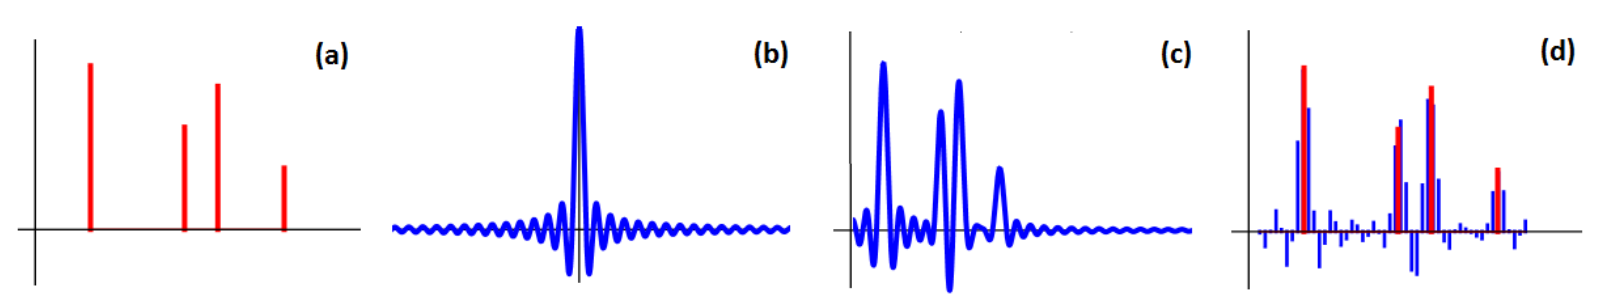
\includegraphics[width=0.8\textwidth]{figures/basismismatch.png}
    %     \\{\addendum{\scriptsize Courtesy of Helena Tukuljac~\cite{tukuljac2018mulan}}}
    %     \\{\small \textcolor{myred}{\iconAlert~sampling breaks sparsity and non-negativity}}
    % \end{center}

\end{frame}